\chapter{Конструкторский раздел}
\label{cha:design}

\section{Схемы алгоритма Левенштейна}
На рисунке ~\ref{fig:rec_lev} приведена схема рекурсивного алгоритма Левенштейна.
На рисунке ~\ref{fig:rec_lev_memo} приведена схема рекрсивного алгоритма Левенштейна с кэшированием.
На рисунке ~\ref{fig:iter_lev} приведена схема итеративного алгоритма Левенштейна.
На рисунке ~\ref{fig:dam_lev} приведена схема итеративного алгоритма Дамерау--Левенштейна.
\begin{figure}
    \centering
    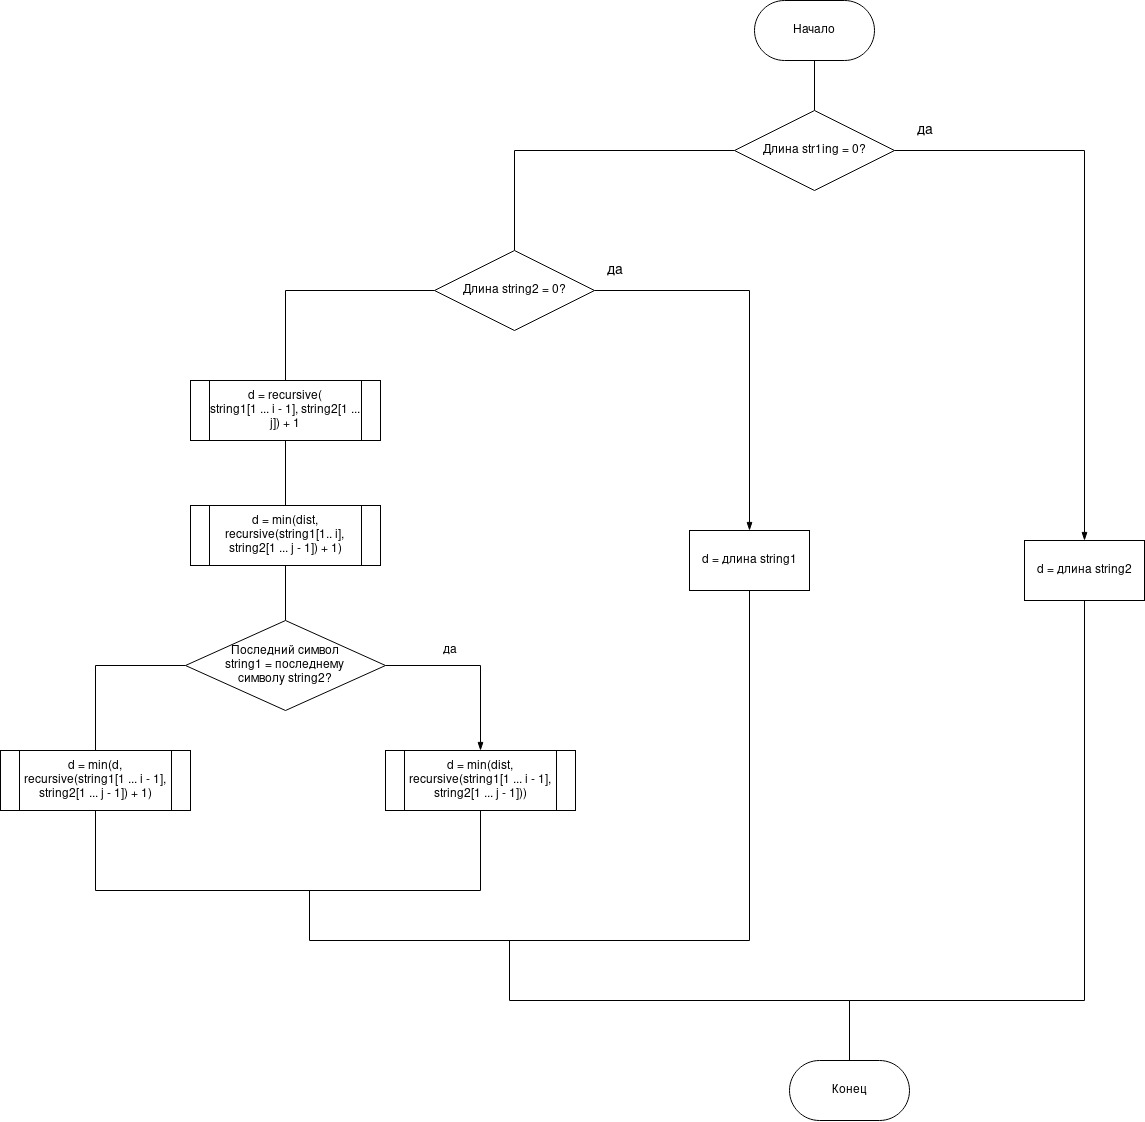
\includegraphics[height=0.65\textheight]{sem-v-aa-master/lab1/tex/inc/schemes/rec.jpg}
    \caption{Схема рекурсивного алгоритма Левенштейна}
    \label{fig:rec_lev}
\end{figure}
\begin{figure}
    \centering
    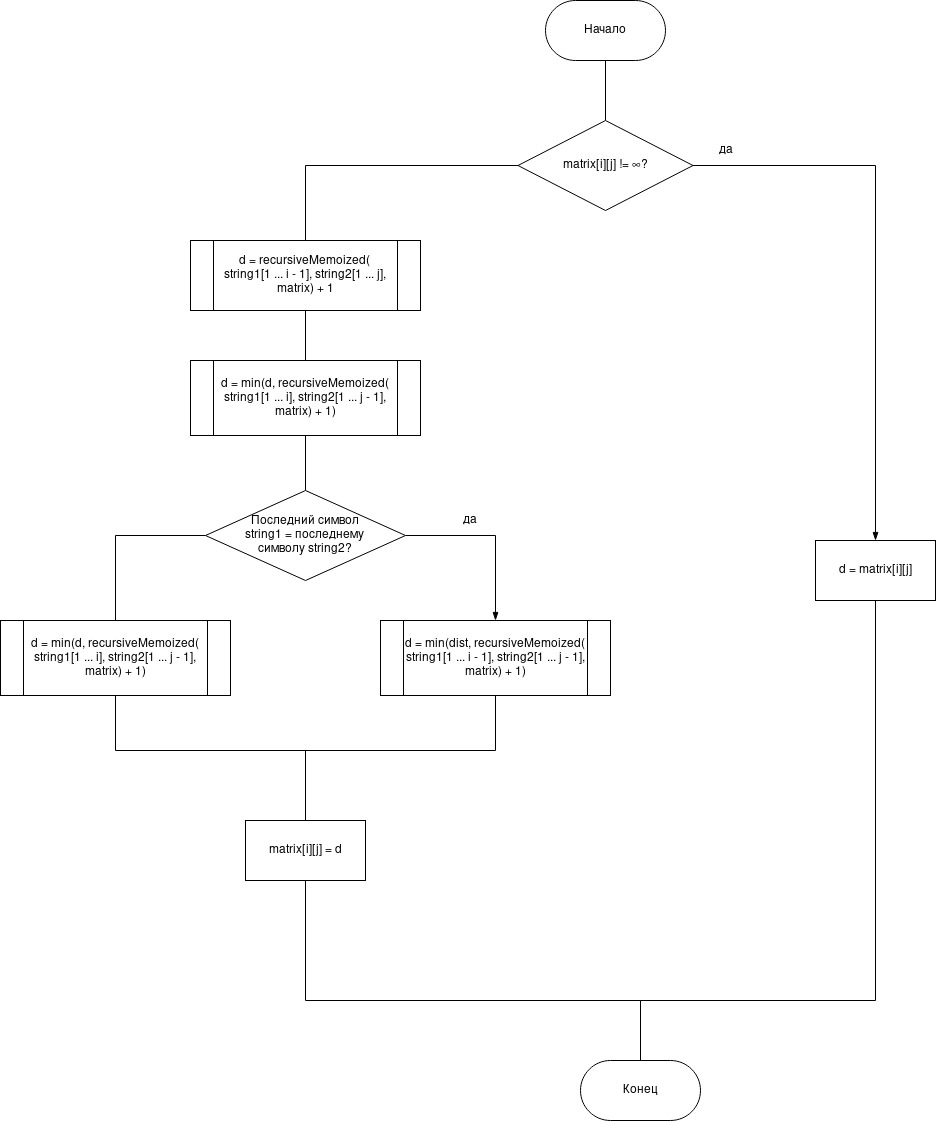
\includegraphics[height=0.65\textheight]{sem-v-aa-master/lab1/tex/inc/schemes/mem.jpg}
    \caption{Схема рекурсивного алгоритма Левенштейна с кэшированием}
    \label{fig:rec_lev_memo}
\end{figure}
\begin{figure}
    \centering
    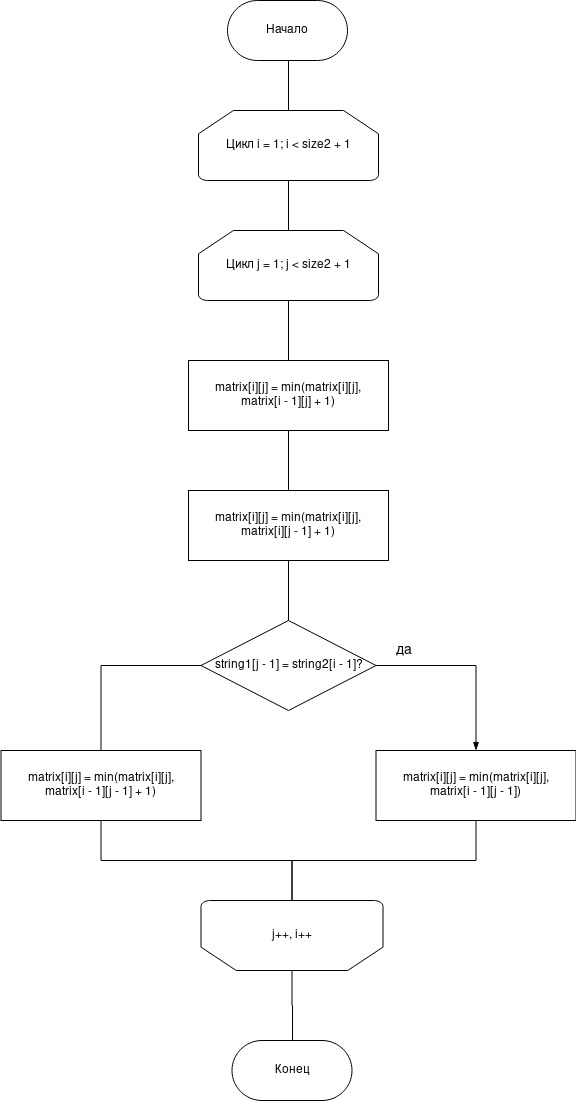
\includegraphics[height=0.65\textheight]{sem-v-aa-master/lab1/tex/inc/schemes/iter.jpg}
    \caption{Схема итеративного алгоритма Левенштейна}
    \label{fig:iter_lev}
\end{figure}
\begin{figure}
    \centering
    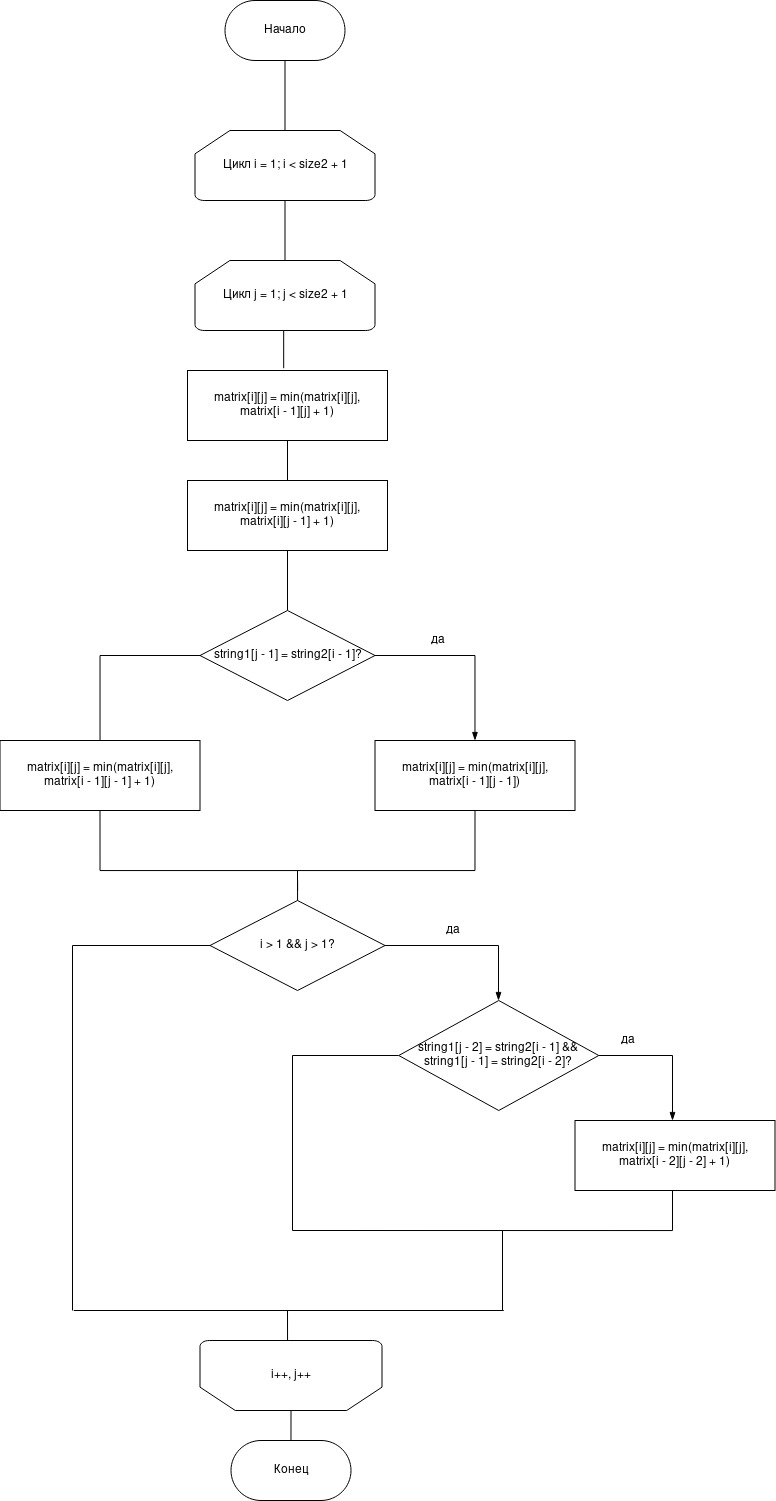
\includegraphics[height=0.65\textheight]{sem-v-aa-master/lab1/tex/inc/schemes/iter_dl.jpg}
    \caption{Схема итеративного алгоритма Дамерау--Левенштейна}
    \label{fig:dam_lev}
\end{figure}

\section{Вывод}

На основе теоретического материала из аналитического раздела были построены схемы реализаций исследуемых алгоритмов.

%%% Local Variables:
%%% mode: latex
%%% TeX-master: "rpz"
%%% End:
